%----------------------------------------------------------------
%
%  File    :  thesis.tex
%
%  Authors :  Keith Andrews, IICM, TU Graz, Austria
%             Manuel Koschuch, FH Campus Wien, Austria
%			  Sebastian Ukleja, FH Campus Wien, Austria
% 
%  Created :  22 Feb 96
% 
%  Changed :  14 Oct 2020
%
%  For suggestions and remarks write to: sebastian.ukleja@fh-campuswien.ac.at 
%----------------------------------------------------------------

% --- Setup for the document ------------------------------------

%Class for a book like style:
\documentclass[11pt,a4paper,oneside]{scrbook}
%For a more paper like style use this class instead:
%\documentclass[11pt,a4paper,oneside]{thesis}

%input encoding for windows in utf-8 needed for Ä,Ö,Ü etc..:
\usepackage[utf8]{inputenc}
%input encoding for linux:
%\usepackage[latin1]{inputenc}
%input encoding for mac:
%\usepackage[applemac]{inputenc}

\usepackage[ngerman]{babel}
%for english use this instead:
%\usepackage[english]{babel}

\usepackage{csquotes}
\MakeOuterQuote{"}

\usepackage{float}

%needed for font encoding
\usepackage[T1]{fontenc}

% want Arial? uncomment next two lines...
%\usepackage{uarial}
%\renewcommand{\familydefault}{\sfdefault}

%some formatting packages
\usepackage[bf,sf]{subfigure}
\renewcommand{\subfigtopskip}{0mm}
\renewcommand{\subfigcapmargin}{0mm}

%For better font resolution in pdf files
\usepackage{lmodern}

\usepackage{url}

%\usepackage{latexsym}

\usepackage{geometry} % define pagesize in more detail

% --- Settings for header and footer ---------------------------------
\usepackage{scrlayer-scrpage}
\clearscrheadfoot
\pagestyle{scrheadings}
\automark{chapter}

%Left header shows chapter and chapter name, will not display on first chapter page use \ihead*{\leftmark} to show on every page
\ihead{\leftmark} 	
%\ohead*{\rightmark}	%optional right header
\ifoot*{Markus Mayer}	%left footer shows student name
\ofoot*{\thepage}		%right footer shows pagination
%---------------------------------------------------------------------

\usepackage{colortbl} % define colored backgrounds for tables

\usepackage{courier} %for listings
\usepackage{listings} % nicer code formatting
\lstset{basicstyle=\ttfamily,breaklines=true}

\usepackage{graphicx}
  \pdfcompresslevel=9
  \pdfpageheight=297mm
  \pdfpagewidth=210mm
  \usepackage[         % hyperref should be last package loaded
    pdftex, 		   % needed for pdf compiling, DO NOT compile with LaTeX
    bookmarks,
    bookmarksnumbered,
    linktocpage,
    pagebackref,
    pdfview={Fit},
    pdfstartview={Fit},
    pdfpagemode=UseOutlines,                 % open bookmarks in Acrobat
  ]{hyperref}
\DeclareGraphicsExtensions{.pdf,.jpg,.png}
\usepackage{bookmark}

\usepackage[title]{appendix}

%paper format
\geometry{a4paper,left=30mm,right=25mm, top=30mm, bottom=30mm}

\setlength{\parskip}{3pt plus 1pt minus 0pt}       % vert. space before a paragraph

\setcounter{tocdepth}{1}        % lowest section level entered in ToC
\setcounter{secnumdepth}{2}     % lowest section level still numbered

%Start of your document beginning with title page
\begin{document}

% --- Main Title Page ------------------------------------------------
\begin{titlepage}
\frontmatter
\begin{picture}(50,50)
\put(-70,40){\hbox{
\includegraphics{images/logo.png}}}
\end{picture}

\vspace*{-5.8cm}

\begin{center}

\vspace{6.2cm}

\hspace*{-1.0cm} {\LARGE \textbf{Titel \\}}
\vspace{0.2cm}
\hspace*{-1.0cm} Untertitel \\

\vspace{2.0cm}

\hspace*{-1.0cm} { \textbf{Bachelorarbeit\\}}

\vspace{0.65cm}

\hspace*{-1.0cm} Eingereicht in teilweiser Erfüllung der Anforderungen zur Erlangung des akademischen Grades: \\

\vspace{0.65cm}

\hspace*{-1.0cm} \textbf{Bachelor of Science in Engineering\\}

\vspace{0.65cm}

\hspace*{-1.0cm} an der FH Campus Wien \\
\vspace{0.2cm}
\hspace*{-1.0cm} Studienfach: Computer Science and Digital Communications \\

\vspace{1.6cm}

\hspace*{-1.0cm} \textbf{Autor:} \\
\vspace{0.2cm}
\hspace*{-1.0cm} Markus Mayer \\

\vspace{0.7cm}

\hspace*{-1.0cm} \textbf{Matrikelnummer:}\\
\vspace{0.2cm}
\hspace*{-1.0cm} 52006537 \\

\vspace{0.7cm}

\hspace*{-1.0cm} \textbf{Betreuer:} \\
\vspace{0.2cm}
\hspace*{-1.0cm} MSc René Goldschmid \\

\vspace{0.7cm}

% Reviewer if needed:
%\hspace*{-1.0cm} \textbf{Reviewer: (optional)} \\
%\vspace{0.2cm}
%\hspace*{-1.0cm} Titel Vorname Nachname \\


\vspace{1.0cm}

\hspace*{-1.0cm} \textbf{Datum:} \\
\vspace{0.2cm}
\hspace*{-1.0cm} 25.09.2022 \\

\end{center}
\end{titlepage}

\newpage

\setcounter{page}{1}

\vspace*{16cm}

% --- Declaration of authorship --------------------------------------------
\hspace*{-0.7cm} \underline{Erklärung der Urheberschaft:}\\\\
Ich erkläre hiermit diese Bachelorarbeit eigenständig verfasst zu haben. Ich habe keine anderen Quellen, als die in der Arbeit gelisteten verwendet, noch habe ich jegliche unerlaubte Hilfe in Anspruch genommen\\\\
Ich versichere diese Bachelorarbeit in keinerlei Form jemandem Anderen oder einer anderen Institution zur Verfügung gestellt zu haben, weder in Österreich noch im Ausland.\\\\
Weiters versichere ich, dass jegliche Kopie (gedruckt oder digital) identisch ist.
\\\\\\
Datum: \hspace{6cm} Unterschrift:\\

% --- English Abstract ----------------------------------------------------
\cleardoublepage
\chapter*{Abstract}
(E.g. ``This thesis investigates...'')


% --- German Abstract ----------------------------------------------------

\cleardoublepage
\chapter*{Kurzfassung}
(Z.B. ``Diese Arbeit untersucht...'')

% --- Abbrevations ----------------------------------------------------
\newpage\noindent
\chapter*{Abkürzungen}
\vspace{0.65cm}

\begin{table*}[htbp]
		\begin{tabular}{ll}
			OHA      & Open Handset Alliance \\
			OAA      & Open Automotive Alliance \\
            LiPS     & Linux Phone Standards Forum  \\
            OMA      & Open Mobile Alliance \\
            IDE      & Integrated Development Enviroment \\
		\end{tabular}
\end{table*}

% --- Key terms ----------------------------------------------------
\newpage
\chapter*{Schlüsselbegriffe}
\vspace{0.65cm}

\begin{itemize}
	\setlength{\itemsep}{0pt}
	\item[] 1
	\item[] 2
	\item[] 3
\end{itemize}

% --- Table of contents autogenerated ------------------------------------
\newpage
\tableofcontents

% --- Begin of Thesis ----------------------------------------------------
\mainmatter
\chapter{Einführung}
\section{Motivation}
Warum ist diese Arbeit interessant?
\section{Relevanz}
Inwiefern ist diese Arbeit neu und wichtig?


\chapter{Hauptteil}

\section{Android-Übersicht}

Um einen Überblick über Android zu bekommen, beziehungsweise wo der Fokus des am weitest verbreitetsten Betriebssystem für mobile Geräte liegt, muss man etwas in die Vergangenheit blicken. Android ist ein Open-Source-Betriebssystem, welches auf einem Linux-Kernel basiert. Es wurde von der Firma Android Inc. entwickelt, die im Jahr 2005 von Google übernommen wurde \cite{hrmoandroid}.


\subsection{Rückblick}

Im Jahr 2006 hatten Hersteller, die ein Smartphone auf den Markt bringen wollten, nur zwei ziemlich teure Möglichkeiten. Entweder Lizenzgebühr für ein Betriebssystem bezahlen oder ein eigenes Betriebssystem entwickeln. Google gründet 2007 die Open Handset Alliance (OHA) und führt Android als Open Source-Plattform ein. Im Jahr 2008 wird Android auf die Version mit dem Namen Cupcake aktualisiert. Bei dieser Version können Hersteller wie HTC und Samsung, aber auch Mobilfunkanbieter das Betriebssystems ihrer Smartphones anpassen. Laut Google kommt 2010 Android auf 34 Mobilgerätetypen in 49 Ländern zum Einsatz und bietet damit den Nutzern eine größere Auswahl als je zuvor. 2011 veröffentlicht Google mit Android 3.0 Honeycomb ein für Tablets optimiertes Betriebssystem, das als Basis für das Betriebssystem Fire OS des Kindle Fire-Tablets von Amazon dient. Der sogenannte Android Market wird 2012 in Google Play umbenannt und Entwickler können weiterhin ihre Apps in wenigen Stunden veröffentlichen. Zusätzlich zur Unterstützung von Mobilgeräten wird 2014 die Open Automotive Alliance (OAA) gegründet, deren Ziel es ist Android auch für Autos zu nutzen. Heute sind 45 führende Automarken Mitglied der OAA. Durch die Innovationskraft einiger Hersteller sind 2015 inzwischen Android Geräte für weniger als 50 US-Dollar verfügbar. Mit Stand 2016 gibt es fast 24.000 Android Geräte von über 1.300 Marken. Außerdem gibt es heute dutzende weltweit operierende Stores für Android-Apps. \cite{android.com}

Androids Ziele sind zwar ähnlich zu denen des Linux Phone Standards Forum (LiPS) oder der Open Mobile Alliance (OMA), da aber der Ansatz des kompletten Software-Stacks von Android weit über den Fokus dieser standarddefinierenden Organisationen hinausgeht, ist Android kein Teil dieser Organisationen. Verglichen mit dem iPhone, dass eine vollständig herstellerspezifische Hardware- und Softwareplattform ist, die von einem einzigen Unternehmen herausgegeben wird, ist Android ein Open Source-Software-Stack, der von der OHA entwickelt und unterstützt wird und auf jedem kompatiblen Gerät funktionieren soll. \cite{meier_hello_android}


\subsection{Programmiersprachen}

Bis 2019 war Java die offizielle Standardprogrammiersprache für die Entwicklung von Android Apps. Als 2017 Kotlin als unterstützte Sprache für die Android Entwicklung angekündigt wurde, gab es zu Beginn große Aufregung unter den Entwicklern. Jedoch ist die Anzahl der Entwickler die Kotlin verwenden in kürzester Zeit so gestiegen, dass im Jahr 2019 Kotlin, Java als offizielle Standardprogrammiersprache ablöste. \cite{ android_kotlin}

Mit Javas Ablöse als Standardprogrammiersprache wurde seitens Android jedoch weiterhin der offizielle Support für Java und C++ zugesichert \cite{ android_languages}.  Das Feedback, dass direkt von den Entwicklern kommt hebt folgende Vorteile bei der Verwendung von Kotlin hervor \cite{developer.android.com/kotlin/first}.

\begin{itemize} 
  \item Ausdrucksstark und prägnant \\ 
        Es kann mit weniger Code mehr erreicht werden. Codesegmente, die ohne Änderung immer wieder verwendet werden, fachsprachlich auch Boilerplate-Code genannt, können merkbar reduziert werden. Somit kann Kotlin die Produktivität der Entwickler erhöhen. 
  \item Sicherer Code \\ 
        Kotlin enthält viele Sprachfunktionen, die dabei helfen häufige Programmierfehler, wie zum Beispiel Null Pointer Exceptions zu vermeiden. Android Apps mit Kotlin Code haben eine 20-prozentige geringer Absturzwahrscheinlichkeit. 
  \item Interoperabel \\ 
        Kotlin zu 100 Prozent interoperabel mit der Programmiersprache Java, das heißt das Java Code in Kotlin verwendet werden kann und Kotlin Code auch problemlos von Java aus verwendet werden kann. Damit können die Entwickler so viel oder so wenig Kotlin Code in ihren Projekten verwenden, wie sie möchten. 
  \item Strukturierte Gleichzeitigkeit \\ 
        Mit Kotlin Coroutines ist das Arbeiten mit asynchronem Code genauso einfach wie mit blockierendem Code. Diese Coroutines vereinfachen die Verwaltung von diversen Hintergrundaufgaben.
\end{itemize}


\subsection{Android Studio}

Android Studio ist seit 2013 die offizielle Integrated Development Environment (IDE) von Google für die Android-Softwareentwicklung. Um Android Studio zu entwickeln, ging Google eine Kooperation mit der tschechischen Firma JetBrains ein, die zu diesem Zeitpunkt mit IntelliJ IDEA eine der fortschrittlichsten Java IDEs am Markt hatten und auch heute noch haben. Android Studio basiert auf dieser leistungsstarken Entwicklungsumgebung, die von Google mit speziellen Funktionen für die Android-Entwicklung erweitert und angepasst wurde. Eine dieser Funktionen ist ein Build-System, das auf Gradle basiert und mit dem Android Gradle Plugin um einige Features erweitert wurde. Die aktuelle Version ist Android Studio Dolphin mit dem Versionscode 2021.3.1. Android Studio ist ein Open Source Projekt und steht auch frei zum Download zur Verfügung. \cite{android_studio}


\subsection{Gradle}




\section{Android Jetpack-Übersicht}

Android Jetpack wurde von der Support Library inspiriert, dabei handelt es sich um eine Reihe von Komponenten, die es erleichtern neue Android Funktionen zu nutzen und dabei trotzdem eine Abwärtskompatibilität aufrecht zu erhalten. Nahezu jede App im Play Store verwendete diese Support Library. Aufgrund dieser Beliebtheit wurden 2017 die Architecture Components eingeführt. Sie erleichtern den Umgang mit Daten bei Änderungen und Komplikationen im Lebenszyklus einer App. Android Jetpack bringt die existierende Support Library und die Architecture Components zusammen und gliedert sie in vier Kategorien, wie in Abbildung \ref{fig:AndroidJetpackUebersicht} zu sehen ist. \cite{android_jetpack_ueberblick}

\begin{figure}[H]
	\centering
		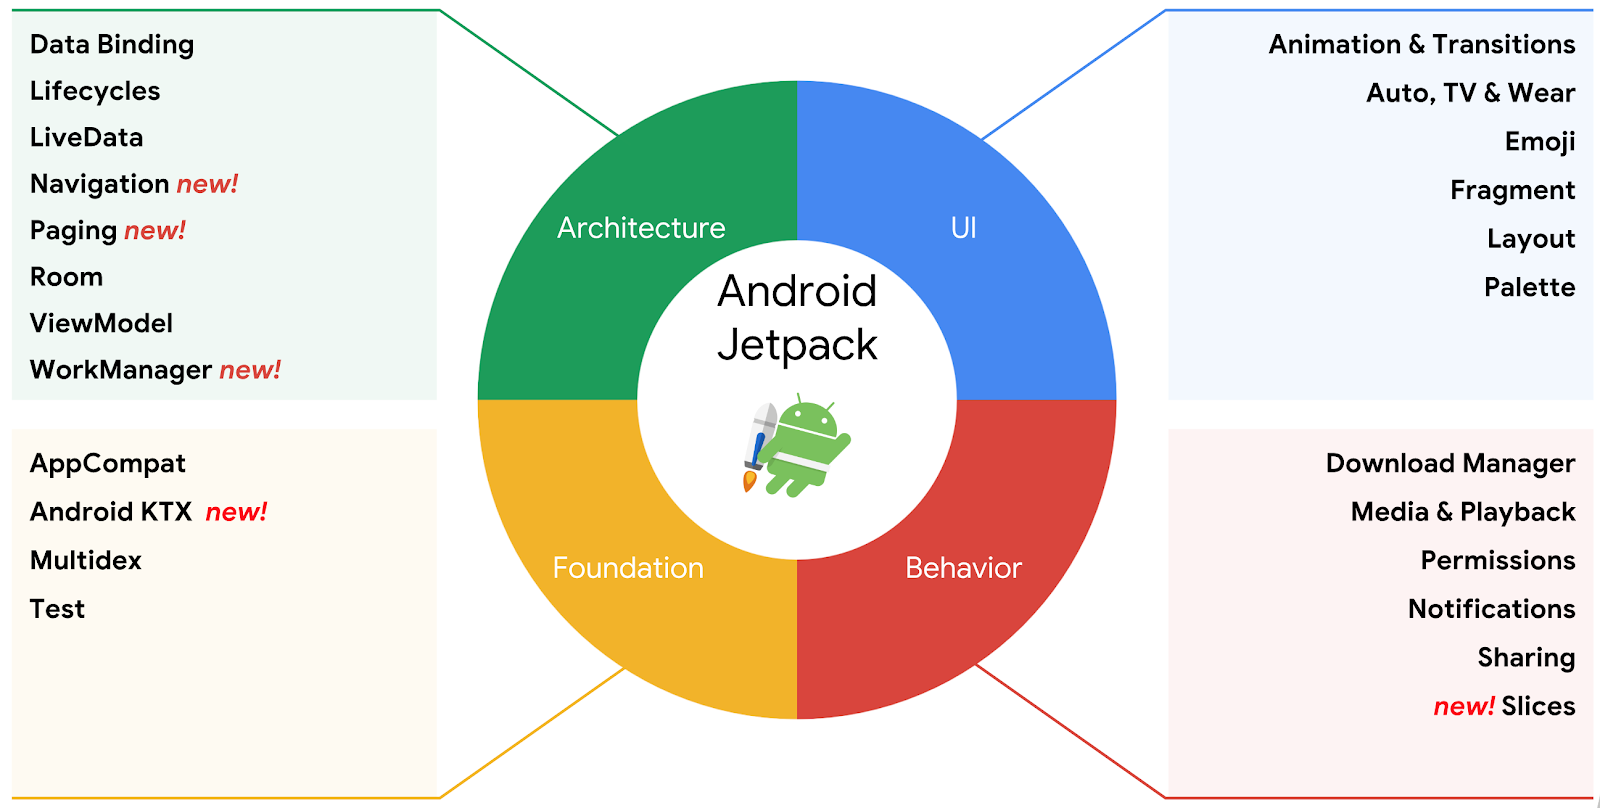
\includegraphics[width=\textwidth]{images/AndroidJetpackUebersicht.png}
	\caption{Überblick über die Komponenten von Android Jetpack \cite{android_jetpack_ueberblick}}
	\label{fig:AndroidJetpackUebersicht}
\end{figure}

Android Jetpack ist eine Sammlung von Bibliotheken und soll Entwicklern dabei helfen, Best Practices zu befolgen, Boilerplate-Code zu reduzieren und Code zu schreiben, der über alle Android-Versionen und -Geräte hinweg konsistent funktioniert \cite{android_jetpack}. Da die Komponenten so aufgebaut sind, dass ihre Funktionalität versionsunabhängig zur Verfügung steht, ist die Abwärtskompatibilität gewährleistet \cite{android_jetpack_ueberblick}. Damit haben Entwickler mehr Zeit sich auf den Code zu konzentrieren, der für ihre App wichtig ist, um leichter und schneller, robuste und hochwertige Apps zu entwickeln. 

Android Jetpack verwaltet also Aktivitäten wie Hintergrundaufgaben, Navigation und Lebenszyklusmanagement. Jetpack ist für eine gute Zusammenarbeit mit Kotlin konzipiert und zusätzlich kann mit der Komponente Android KTX einiges an Code eingespart werden. Die von Jetpack verwalteten Aktivitäten, Kotlin und die Komponenten Android KTX tragen daher gemeinsam dazu bei den Boilerplate-Code zu eliminieren. \cite{android_whats_new}

Die Android Jetpack Komponenten sind als sogenannte "unbundled" Libraries bereitgestellt und sind nicht Teil der Android-Plattform. Dadurch können Updates der Libraries auch unabhängig und öfter durchgeführt werden \cite{androidx_releases}. Diese Libraries wurden alle in den neuen androidx.* Namespace verschoben und können einzeln oder auch in Kombination verwendet werden. \cite{android_jetpack_ueberblick} Daher ist AndroidX eine wesentliche Verbesserung zu der ursprünglichen Android Support Library, welche nicht mehr gewartet wird \cite{androidx_ueberblick}.


\section{Android Jetpack-Komponenten}
\subsection{Core}
\subsection{Activity}
\subsection{Lifecycle}
\subsection{Compose}
\subsection{Navigation}
\subsection{Room}


\chapter{Schluss}
\section{Zusammenfassung}
Wichtigsten Aussagen der Arbeit wiederholen und miteinander in Beziehung bringen

\section{Bewertung und Ausblick}
Bewertung der verschiedenen Faktoren und Erkenntnisse \\
Ideen für weitere Arbeiten

\newpage

% --- Bibliography ------------------------------------------------------

%IEEE Citation [1]:
\bibliographystyle{IEEEtran}
%for alphanumeric citation eg.: [ABC19]
%\bibliographystyle{alpha}

% List references I definitely want in the bibliography,
% regardless of whether or not I cite them in the thesis.

\newpage
\addcontentsline{toc}{chapter}{Bibliographie}
\bibliography{thesis}

\newpage

% --- List of Figures ----------------------------------------------------

\addcontentsline{toc}{chapter}{Abbildungen}
\listoffigures


% --- List of Tables -----------------------------------------------------

\newpage
\addcontentsline{toc}{chapter}{Tabellen}
\listoftables

% --- Appendix A -----------------------------------------------------

\newpage
\backmatter
\appendix
\begin{appendices}
\chapter{Appendix}

(Hier können Schaltpläne, Programme usw. eingefügt werden.)

\clearpage
\end{appendices}

\end{document}
